\documentclass[twoside]{book}

% Packages required by doxygen
\usepackage{fixltx2e}
\usepackage{calc}
\usepackage{doxygen}
\usepackage[export]{adjustbox} % also loads graphicx
\usepackage{graphicx}
\usepackage[utf8]{inputenc}
\usepackage{makeidx}
\usepackage{multicol}
\usepackage{multirow}
\PassOptionsToPackage{warn}{textcomp}
\usepackage{textcomp}
\usepackage[nointegrals]{wasysym}
\usepackage[table]{xcolor}

% Font selection
\usepackage[T1]{fontenc}
\usepackage[scaled=.90]{helvet}
\usepackage{courier}
\usepackage{amssymb}
\usepackage{sectsty}
\renewcommand{\familydefault}{\sfdefault}
\allsectionsfont{%
  \fontseries{bc}\selectfont%
  \color{darkgray}%
}
\renewcommand{\DoxyLabelFont}{%
  \fontseries{bc}\selectfont%
  \color{darkgray}%
}
\newcommand{\+}{\discretionary{\mbox{\scriptsize$\hookleftarrow$}}{}{}}

% Page & text layout
\usepackage{geometry}
\geometry{%
  a4paper,%
  top=2.5cm,%
  bottom=2.5cm,%
  left=2.5cm,%
  right=2.5cm%
}
\tolerance=750
\hfuzz=15pt
\hbadness=750
\setlength{\emergencystretch}{15pt}
\setlength{\parindent}{0cm}
\setlength{\parskip}{3ex plus 2ex minus 2ex}
\makeatletter
\renewcommand{\paragraph}{%
  \@startsection{paragraph}{4}{0ex}{-1.0ex}{1.0ex}{%
    \normalfont\normalsize\bfseries\SS@parafont%
  }%
}
\renewcommand{\subparagraph}{%
  \@startsection{subparagraph}{5}{0ex}{-1.0ex}{1.0ex}{%
    \normalfont\normalsize\bfseries\SS@subparafont%
  }%
}
\makeatother

% Headers & footers
\usepackage{fancyhdr}
\pagestyle{fancyplain}
\fancyhead[LE]{\fancyplain{}{\bfseries\thepage}}
\fancyhead[CE]{\fancyplain{}{}}
\fancyhead[RE]{\fancyplain{}{\bfseries\leftmark}}
\fancyhead[LO]{\fancyplain{}{\bfseries\rightmark}}
\fancyhead[CO]{\fancyplain{}{}}
\fancyhead[RO]{\fancyplain{}{\bfseries\thepage}}
\fancyfoot[LE]{\fancyplain{}{}}
\fancyfoot[CE]{\fancyplain{}{}}
\fancyfoot[RE]{\fancyplain{}{\bfseries\scriptsize Generated by Doxygen }}
\fancyfoot[LO]{\fancyplain{}{\bfseries\scriptsize Generated by Doxygen }}
\fancyfoot[CO]{\fancyplain{}{}}
\fancyfoot[RO]{\fancyplain{}{}}
\renewcommand{\footrulewidth}{0.4pt}
\renewcommand{\chaptermark}[1]{%
  \markboth{#1}{}%
}
\renewcommand{\sectionmark}[1]{%
  \markright{\thesection\ #1}%
}

% Indices & bibliography
\usepackage{natbib}
\usepackage[titles]{tocloft}
\setcounter{tocdepth}{3}
\setcounter{secnumdepth}{5}
\makeindex

% Hyperlinks (required, but should be loaded last)
\usepackage{ifpdf}
\ifpdf
  \usepackage[pdftex,pagebackref=true]{hyperref}
\else
  \usepackage[ps2pdf,pagebackref=true]{hyperref}
\fi
\hypersetup{%
  colorlinks=true,%
  linkcolor=blue,%
  citecolor=blue,%
  unicode%
}

% Custom commands
\newcommand{\clearemptydoublepage}{%
  \newpage{\pagestyle{empty}\cleardoublepage}%
}

\usepackage{caption}
\captionsetup{labelsep=space,justification=centering,font={bf},singlelinecheck=off,skip=4pt,position=top}

%===== C O N T E N T S =====

\begin{document}

% Titlepage & ToC
\hypersetup{pageanchor=false,
             bookmarksnumbered=true,
             pdfencoding=unicode
            }
\pagenumbering{alph}
\begin{titlepage}
\vspace*{7cm}
\begin{center}%
{\Large Kalkulator }\\
\vspace*{1cm}
{\large Generated by Doxygen 1.8.14}\\
\end{center}
\end{titlepage}
\clearemptydoublepage
\pagenumbering{roman}
\tableofcontents
\clearemptydoublepage
\pagenumbering{arabic}
\hypersetup{pageanchor=true}

%--- Begin generated contents ---
\chapter{Namespace Index}
\section{Packages}
Here are the packages with brief descriptions (if available)\+:\begin{DoxyCompactList}
\item\contentsline{section}{\mbox{\hyperlink{namespace_kalkulator}{Kalkulator}} }{\pageref{namespace_kalkulator}}{}
\item\contentsline{section}{\mbox{\hyperlink{namespace_my_calculatorv1}{My\+Calculatorv1}} }{\pageref{namespace_my_calculatorv1}}{}
\end{DoxyCompactList}

\chapter{Hierarchical Index}
\section{Class Hierarchy}
This inheritance list is sorted roughly, but not completely, alphabetically\+:\begin{DoxyCompactList}
\item Application\begin{DoxyCompactList}
\item \contentsline{section}{Kalkulator.\+App}{\pageref{class_kalkulator_1_1_app}}{}
\end{DoxyCompactList}
\item Window\begin{DoxyCompactList}
\item \contentsline{section}{My\+Calculatorv1.\+Main\+Window}{\pageref{class_my_calculatorv1_1_1_main_window}}{}
\end{DoxyCompactList}
\end{DoxyCompactList}

\chapter{Class Index}
\section{Class List}
Here are the classes, structs, unions and interfaces with brief descriptions\+:\begin{DoxyCompactList}
\item\contentsline{section}{\mbox{\hyperlink{class_kalkulator_1_1_app}{Kalkulator.\+App}} \\*Logika interakcji dla klasy App.\+xaml }{\pageref{class_kalkulator_1_1_app}}{}
\item\contentsline{section}{\mbox{\hyperlink{class_my_calculatorv1_1_1_main_window}{My\+Calculatorv1.\+Main\+Window}} }{\pageref{class_my_calculatorv1_1_1_main_window}}{}
\end{DoxyCompactList}

\chapter{Namespace Documentation}
\hypertarget{namespace_kalkulator}{}\section{Kalkulator Namespace Reference}
\label{namespace_kalkulator}\index{Kalkulator@{Kalkulator}}
\subsection*{Classes}
\begin{DoxyCompactItemize}
\item 
class \mbox{\hyperlink{class_kalkulator_1_1_app}{App}}
\begin{DoxyCompactList}\small\item\em Logika interakcji dla klasy App.\+xaml \end{DoxyCompactList}\end{DoxyCompactItemize}

\hypertarget{namespace_my_calculatorv1}{}\section{My\+Calculatorv1 Namespace Reference}
\label{namespace_my_calculatorv1}\index{My\+Calculatorv1@{My\+Calculatorv1}}
\subsection*{Classes}
\begin{DoxyCompactItemize}
\item 
class \mbox{\hyperlink{class_my_calculatorv1_1_1_main_window}{Main\+Window}}
\end{DoxyCompactItemize}

\chapter{Class Documentation}
\hypertarget{class_kalkulator_1_1_app}{}\section{Kalkulator.\+App Class Reference}
\label{class_kalkulator_1_1_app}\index{Kalkulator.\+App@{Kalkulator.\+App}}


Logika interakcji dla klasy App.\+xaml  


Inheritance diagram for Kalkulator.\+App\+:\begin{figure}[H]
\begin{center}
\leavevmode
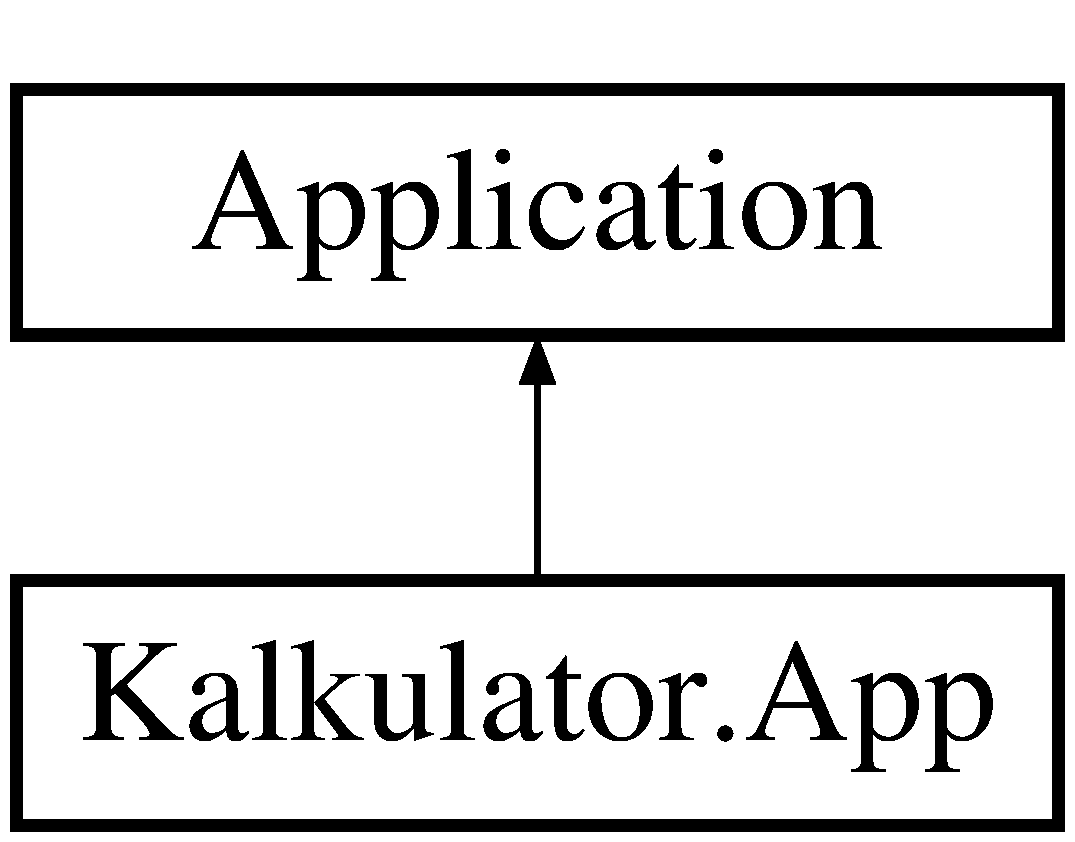
\includegraphics[height=2.000000cm]{class_kalkulator_1_1_app}
\end{center}
\end{figure}


\subsection{Detailed Description}
Logika interakcji dla klasy App.\+xaml 



The documentation for this class was generated from the following file\+:\begin{DoxyCompactItemize}
\item 
C\+:/\+Users/\+Sebek/\+Desktop/\+Kalkulator/\+Kalkulator/App.\+xaml.\+cs\end{DoxyCompactItemize}

\hypertarget{class_my_calculatorv1_1_1_main_window}{}\section{My\+Calculatorv1.\+Main\+Window Class Reference}
\label{class_my_calculatorv1_1_1_main_window}\index{My\+Calculatorv1.\+Main\+Window@{My\+Calculatorv1.\+Main\+Window}}
Inheritance diagram for My\+Calculatorv1.\+Main\+Window\+:\begin{figure}[H]
\begin{center}
\leavevmode
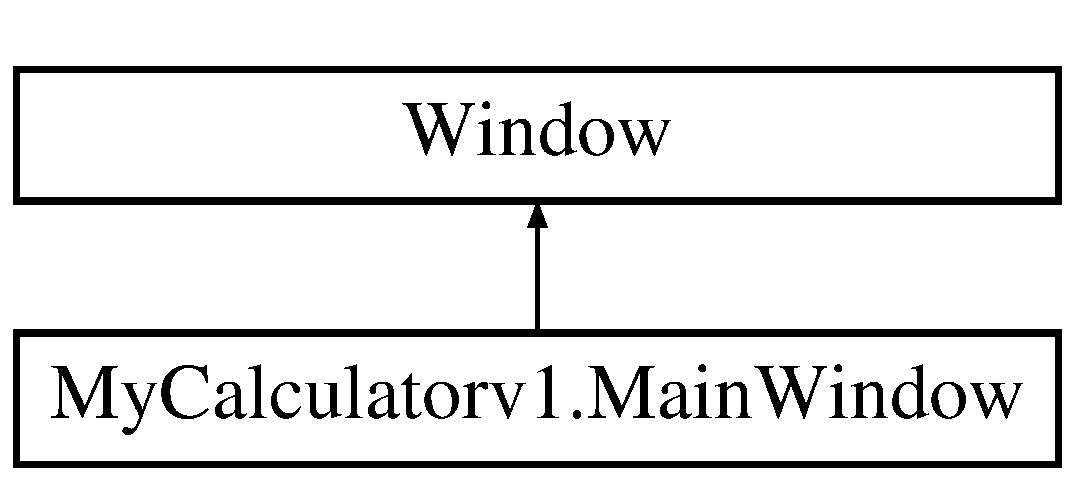
\includegraphics[height=2.000000cm]{class_my_calculatorv1_1_1_main_window}
\end{center}
\end{figure}
\subsection*{Private Member Functions}
\begin{DoxyCompactItemize}
\item 
void \mbox{\hyperlink{class_my_calculatorv1_1_1_main_window_aeb46937c128a2025721bf75e21c45d3b}{Button\+\_\+\+Click\+\_\+1}} (object sender, Routed\+Event\+Args e)
\begin{DoxyCompactList}\small\item\em Metoda pobierająca wartość wciśniętego przycisku i dopisaniu go na wyświetlaczu \end{DoxyCompactList}\item 
void \mbox{\hyperlink{class_my_calculatorv1_1_1_main_window_a6c07df3d7d2ac3eb3218f01a2f3de9c6}{Result\+\_\+click}} (object sender, Routed\+Event\+Args e)
\item 
void \mbox{\hyperlink{class_my_calculatorv1_1_1_main_window_ad2ba19ce602b4bd65b01bc3c2e44d853}{result}} ()
\begin{DoxyCompactList}\small\item\em Metoda która dokonuje obliczeń w zależności od wybranego znaku. Wyświetla na ekranie przeprowadzone działanie \end{DoxyCompactList}\item 
void \mbox{\hyperlink{class_my_calculatorv1_1_1_main_window_a21ab4fba529eb56956dd8fe73bb7221a}{Off\+\_\+\+Click\+\_\+1}} (object sender, Routed\+Event\+Args e)
\begin{DoxyCompactList}\small\item\em Metoda mająca na celu wyłączyć aplikację \end{DoxyCompactList}\item 
void \mbox{\hyperlink{class_my_calculatorv1_1_1_main_window_a16fceaf60e1a42e3377c49b7266e339b}{Del\+\_\+\+Click}} (object sender, Routed\+Event\+Args e)
\begin{DoxyCompactList}\small\item\em Metoda mająca na celu usunąć wyświetlony tekst \end{DoxyCompactList}\item 
void \mbox{\hyperlink{class_my_calculatorv1_1_1_main_window_a16f87a39b16c90c644dc32632f73a86c}{R\+\_\+\+Click}} (object sender, Routed\+Event\+Args e)
\begin{DoxyCompactList}\small\item\em Metoda usuwająca ostatnio wpisany znak \end{DoxyCompactList}\end{DoxyCompactItemize}


\subsection{Member Function Documentation}
\mbox{\Hypertarget{class_my_calculatorv1_1_1_main_window_aeb46937c128a2025721bf75e21c45d3b}\label{class_my_calculatorv1_1_1_main_window_aeb46937c128a2025721bf75e21c45d3b}} 
\index{My\+Calculatorv1\+::\+Main\+Window@{My\+Calculatorv1\+::\+Main\+Window}!Button\+\_\+\+Click\+\_\+1@{Button\+\_\+\+Click\+\_\+1}}
\index{Button\+\_\+\+Click\+\_\+1@{Button\+\_\+\+Click\+\_\+1}!My\+Calculatorv1\+::\+Main\+Window@{My\+Calculatorv1\+::\+Main\+Window}}
\subsubsection{\texorpdfstring{Button\+\_\+\+Click\+\_\+1()}{Button\_Click\_1()}}
{\footnotesize\ttfamily void My\+Calculatorv1.\+Main\+Window.\+Button\+\_\+\+Click\+\_\+1 (\begin{DoxyParamCaption}\item[{object}]{sender,  }\item[{Routed\+Event\+Args}]{e }\end{DoxyParamCaption})\hspace{0.3cm}{\ttfamily [private]}}



Metoda pobierająca wartość wciśniętego przycisku i dopisaniu go na wyświetlaczu 

\mbox{\Hypertarget{class_my_calculatorv1_1_1_main_window_a16fceaf60e1a42e3377c49b7266e339b}\label{class_my_calculatorv1_1_1_main_window_a16fceaf60e1a42e3377c49b7266e339b}} 
\index{My\+Calculatorv1\+::\+Main\+Window@{My\+Calculatorv1\+::\+Main\+Window}!Del\+\_\+\+Click@{Del\+\_\+\+Click}}
\index{Del\+\_\+\+Click@{Del\+\_\+\+Click}!My\+Calculatorv1\+::\+Main\+Window@{My\+Calculatorv1\+::\+Main\+Window}}
\subsubsection{\texorpdfstring{Del\+\_\+\+Click()}{Del\_Click()}}
{\footnotesize\ttfamily void My\+Calculatorv1.\+Main\+Window.\+Del\+\_\+\+Click (\begin{DoxyParamCaption}\item[{object}]{sender,  }\item[{Routed\+Event\+Args}]{e }\end{DoxyParamCaption})\hspace{0.3cm}{\ttfamily [private]}}



Metoda mająca na celu usunąć wyświetlony tekst 

\mbox{\Hypertarget{class_my_calculatorv1_1_1_main_window_a21ab4fba529eb56956dd8fe73bb7221a}\label{class_my_calculatorv1_1_1_main_window_a21ab4fba529eb56956dd8fe73bb7221a}} 
\index{My\+Calculatorv1\+::\+Main\+Window@{My\+Calculatorv1\+::\+Main\+Window}!Off\+\_\+\+Click\+\_\+1@{Off\+\_\+\+Click\+\_\+1}}
\index{Off\+\_\+\+Click\+\_\+1@{Off\+\_\+\+Click\+\_\+1}!My\+Calculatorv1\+::\+Main\+Window@{My\+Calculatorv1\+::\+Main\+Window}}
\subsubsection{\texorpdfstring{Off\+\_\+\+Click\+\_\+1()}{Off\_Click\_1()}}
{\footnotesize\ttfamily void My\+Calculatorv1.\+Main\+Window.\+Off\+\_\+\+Click\+\_\+1 (\begin{DoxyParamCaption}\item[{object}]{sender,  }\item[{Routed\+Event\+Args}]{e }\end{DoxyParamCaption})\hspace{0.3cm}{\ttfamily [private]}}



Metoda mająca na celu wyłączyć aplikację 

\mbox{\Hypertarget{class_my_calculatorv1_1_1_main_window_a16f87a39b16c90c644dc32632f73a86c}\label{class_my_calculatorv1_1_1_main_window_a16f87a39b16c90c644dc32632f73a86c}} 
\index{My\+Calculatorv1\+::\+Main\+Window@{My\+Calculatorv1\+::\+Main\+Window}!R\+\_\+\+Click@{R\+\_\+\+Click}}
\index{R\+\_\+\+Click@{R\+\_\+\+Click}!My\+Calculatorv1\+::\+Main\+Window@{My\+Calculatorv1\+::\+Main\+Window}}
\subsubsection{\texorpdfstring{R\+\_\+\+Click()}{R\_Click()}}
{\footnotesize\ttfamily void My\+Calculatorv1.\+Main\+Window.\+R\+\_\+\+Click (\begin{DoxyParamCaption}\item[{object}]{sender,  }\item[{Routed\+Event\+Args}]{e }\end{DoxyParamCaption})\hspace{0.3cm}{\ttfamily [private]}}



Metoda usuwająca ostatnio wpisany znak 

\mbox{\Hypertarget{class_my_calculatorv1_1_1_main_window_ad2ba19ce602b4bd65b01bc3c2e44d853}\label{class_my_calculatorv1_1_1_main_window_ad2ba19ce602b4bd65b01bc3c2e44d853}} 
\index{My\+Calculatorv1\+::\+Main\+Window@{My\+Calculatorv1\+::\+Main\+Window}!result@{result}}
\index{result@{result}!My\+Calculatorv1\+::\+Main\+Window@{My\+Calculatorv1\+::\+Main\+Window}}
\subsubsection{\texorpdfstring{result()}{result()}}
{\footnotesize\ttfamily void My\+Calculatorv1.\+Main\+Window.\+result (\begin{DoxyParamCaption}{ }\end{DoxyParamCaption})\hspace{0.3cm}{\ttfamily [private]}}



Metoda która dokonuje obliczeń w zależności od wybranego znaku. Wyświetla na ekranie przeprowadzone działanie 

\mbox{\Hypertarget{class_my_calculatorv1_1_1_main_window_a6c07df3d7d2ac3eb3218f01a2f3de9c6}\label{class_my_calculatorv1_1_1_main_window_a6c07df3d7d2ac3eb3218f01a2f3de9c6}} 
\index{My\+Calculatorv1\+::\+Main\+Window@{My\+Calculatorv1\+::\+Main\+Window}!Result\+\_\+click@{Result\+\_\+click}}
\index{Result\+\_\+click@{Result\+\_\+click}!My\+Calculatorv1\+::\+Main\+Window@{My\+Calculatorv1\+::\+Main\+Window}}
\subsubsection{\texorpdfstring{Result\+\_\+click()}{Result\_click()}}
{\footnotesize\ttfamily void My\+Calculatorv1.\+Main\+Window.\+Result\+\_\+click (\begin{DoxyParamCaption}\item[{object}]{sender,  }\item[{Routed\+Event\+Args}]{e }\end{DoxyParamCaption})\hspace{0.3cm}{\ttfamily [private]}}





Metoda wywołująca \mbox{\hyperlink{class_my_calculatorv1_1_1_main_window_ad2ba19ce602b4bd65b01bc3c2e44d853}{result}}. W przypadku błędu wypisuje na wyświetlaczu Error 

The documentation for this class was generated from the following file\+:\begin{DoxyCompactItemize}
\item 
C\+:/\+Users/\+Sebek/\+Desktop/\+Kalkulator/\+Kalkulator/Main\+Window.\+xaml.\+cs\end{DoxyCompactItemize}

%--- End generated contents ---

% Index
\backmatter
\newpage
\phantomsection
\clearemptydoublepage
\addcontentsline{toc}{chapter}{Index}
\printindex

\end{document}
